\documentclass[a4paper]{article}

\usepackage[english]{babel} \usepackage[colorlinks=true]{hyperref} \usepackage{float}
\usepackage[utf8]{inputenc} \usepackage{amsmath} \usepackage{graphicx}
\usepackage[colorinlistoftodos]{todonotes} \usepackage{tikz}
\usepackage{pdfpages} \usepackage{listings}
\usepackage{listings}
\usepackage{color}
\usepackage{framed,enumitem}



\definecolor{green}{rgb}{0,0.6,0}
\definecolor{gray}{rgb}{0.5,0.5,0.5}
\definecolor{mauve}{rgb}{0.58,0,0.82}


\lstset{frame=tb,
  language=Java,
  aboveskip=3mm,
  belowskip=3mm,
  showstringspaces=false,
  columns=flexible,
  basicstyle={\small\ttfamily},
  numbers=left,
  numberstyle=\tiny\color{gray},
  commentstyle=\color{green},
  stringstyle=\color{mauve},
  breaklines=true,
  breakatwhitespace=true,
  tabsize=3
}
% add above keywordstyle=\color{blue},

\lstset{emph={%  
    for%
    },emphstyle={\color{blue}\bfseries}%
}%

\lstset{escapeinside={(*@}{@*)}}

\renewcommand{\lstlistingname}{Algorithm}

\usetikzlibrary{arrows,positioning,shapes.geometric}

\title{Dynamic A* on \emph{GPU}}
\usepackage{listings}
\usepackage{color}


\author{\normalsize Lokesh Koshale (CS15B049) \\\normalsize}

\date{\color{black}August 23 2019}

\begin{document} \maketitle


% \section{Abstract}
%  We propose algorithm and techniques to solve the dynamic A star guided search on GPU.
% The goal of a dynamic graph algorithm is to
% support query and update operations as
% quickly as possible.

% In many applications graphs are subject to discrete changes, such as additions or deletions
% of edges or vertices.

% The goal of
% a dynamic graph algorithm is to update efficiently the solution of a problem after dynamic changes,
% rather than having to recompute it from scratch each time

\section{Introduction}
A*\cite{A*}\cite{Wiki A*} is one of widely used path planning and shortest path approximation algorithm. It is used widespread due to its performance and accuracy. It is used to find shortest path in maps and games where hindrances can be present. In most of the real life cases graph is not static but it is constantly changing. D*\cite{original D*}, focused D*\cite{focused D*} and D* lite\cite{D* Lite} are a family of informed incremental search algorithm where edge cost can change while we try to find the optimal path. Here we approach the problem where edges can be inserted OR deleted from the graph while the number of nodes are fixed. We assume that graph doesn't change while we are finding the optimal path.\\

\begin{lstlisting}[language=C , caption=A*\cite{A*} ]
Input: A Graph(V,E) with source node (*@\textit{start}@*) and goal node (*@\textit{end}@*).
Output: Least cost path from (*@\textit{start}@*) to (*@\textit{end}@*).
Steps:
Initialize 
    open_list = {(*@\textit{start}@*)}          /* list of nodes to be traversed */
    closed_list = {}              /* list of already traversed node */
    g(start) = 0                  /* cost from source node to node */
    h(start) = heuristic_function(start,end) /* estimated cost from source to goal node */
    f(start) = g(start) + h(start)      /* total cost from goal to node */
    
    while open_list is not empty:
        m = node on top of open_list with least f
        if m == end
            return
        remove m from open_list
        add m to close list
        
        for each n in child(m):
            cost = g(m) + distance(m,n)
            
            if n in open_list and cost < g(n):
                remove n from open_list as new path is better.
                
            if n in closed_list and cost < g(n):
                remove n from closed_list
                
            if n is not in open_list and closed_list:
                g(n) = cost
                h(n) = heuristic_function(n,end)
                f(n) = g(n) + h(n)
                add n to open_list
    
    return failure
    
\end{lstlisting}
General purpose computation on graphics processing units (GPGPU) has been widely used to accelerate numerous computational task. In multicore systems to improve the performance one has to increase the number of cores and adding more and more cores increase the cost thus GPU is an as cost efficient alternative hardware to execute parallel algorithms which also provides better performance. In paper \textit{Massively Parallel A* Search on a GPU}\cite{GA*} the authors proposed a parallel variant of A* for GPU, we borrow the parallelization of A* on GPU from them. The bottle neck for parallelization is the sequential nature of Priority Queue which is the primary data structure to implement A*, to utilise the many core GPU architecture the authors proposed to have multiple priority queues thus expanding many nodes at once. In the paper author claims that GA* gives 30x-45x performance improvement from the CPU implementation.
\begin{lstlisting}[language=FORTRAN, caption=GA*]
procedure GA*(s,t,k)   !find the shortest path from s to t with k queues
Let (*@$\{Q_i\}^k_{i=1} $@*) be the priority queues of open_list
Let H be the closed list
PUSH((*@$Q_1$@*), s)
m (*@$\leftarrow$@*) nil         !m stores the best target state
while (*@$Q$@*) is not empty do:
    Let (*@$S$@*) be an empty list
    for i (*@$\leftarrow$@*) 1 to k in parallel do:
        if (*@$Q_i$@*) is empty then
            continue
        end if
        (*@$q_i \leftarrow$@*) Extract((*@$Q_i$@*))
        if (*@$q_i.node = t$@*) then:
            if m = nil or (*@$f(q_i) < f(m)$@*) then:
                m (*@$\leftarrow q_i$@*)
            end if
            continue
        end if
        (*@$S \leftarrow S + EXPAND(q_i)$@*)
    end for
    
    if m (*@$\neq$@*) nil and (*@$f(m) \leq min_{q\in Q}f(q)$@*) then:
        return the path generated from m
    end if

    (*@$T \leftarrow S$@*)
    for (*@$s'\in S$@*) in parallel do:
        if (*@$s'.node \in H$ @*) and (*@$H[s'.node].g < s'.g$@*) then:
            remove (*@$s'$@*) from (*@$T$@*)
        end if
    end for
    
    for (*@$t' \in T$@*) in parallel do:
        (*@$t'.f \leftarrow f(t')$@*)
        PUSH (*@$t'$@*) to one of priority queues
        (*@$H[t'.node] \leftarrow t'$@*)
    end for
end while

end procedure

\end{lstlisting}
Below are some terminology we will be using in this document.\\
\textbf{Terminology:}
\begin{itemize}
    \item $g(n)$: cost of reaching node $n$ from source
    \item $h(n)$: approximate cost of reaching destination from node $n$
    \item $f(n)$: approximate cost of reaching destination from source via node $n$ $f(n) = g(n) + h(n)$
    \item $w_{uv}$: weight associated with the edge $u \rightarrow v$
    \item open\_list : list of nodes to be traversed.
    \item update\_list: list of nodes to be traversed while doing propagation.
    \item optimal\_cost: same as $f(n)$
    \item optimal\_parent: back edge to the parent from which optimal cost is calculated
    \item Optimal\_Path: source to destination optimal path, which can be traced by following optimal\_parent from destination
    \item $f(n)_{old}$: approximate cost of reaching destination from source via node $n$ before updates (insertion/deletion)
    \item $f(n)_{new}$: approximate cost of reaching destination from source via node $n$ after updates (insertion/deletion)
\end{itemize}
% \section{Properties of A*}
We make certain claims and prove them, which will be later useful in deriving some major algorithmic choices for processing addition and deletion of edges.\\
\\
\hypertarget{Lemma 1}{\textbf{Lemma 1:}}\textit{If we have found a node $d$ which have cost $f_d$ then all the nodes $i \in V$ which have have cost $f_i < f_d$ are already visited(expanded).}\\
\textbf{Proof:} Suppose we found the node $d$ with cost $f_d$ and there exists a node n such that node $n$ is not visited i.e $n \notin closed\_list$ and $f_n < f_d$\\
If $n \notin closed\_list$ then either node $n \in open\_list$ or $n$ is not explored yet which means $f_n = \infty $.\\
If $n \in open\_list$  and we know that $f_n < f_d$, In A* to expand a node we always chose the node with least $f$ ( as in line no 15 of Algorithm 1:A*).So $n$ should be chosen before $d$ and which implies that $n$ is already visited(expanded). which contradicts our assumption that $n$ is not visited.\\
If $f_n = \infty $, we have found the node $d$ so $f_d \neq \infty$ which implies $f_n > f_d$ which violates our assumption that $f_n <  f_d$.\\
hence proved.\\
\textbf{corollary:}\textit{If some nodes are not visited at the end of A* then the optimal cost of all those node will be greater than or equal to the cost of destination. }

\section{Incremental}
In Incremental setting there are only edge-insertions, i.e edge $u \rightarrow v $ is added in G where $u\in V $ and $v \in V$.\\
\\
\begin{center}
    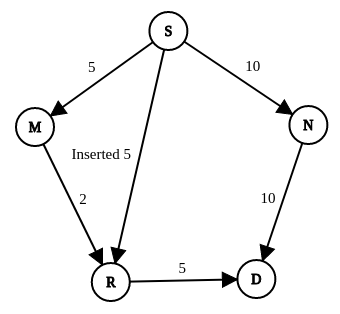
\includegraphics[scale=0.4]{img/insert1.png}
\end{center}
In the above graph the Optimal Path before insertion was $S \rightarrow M \rightarrow R \rightarrow D$, when we insert edge $S \rightarrow D$, the cost $f$ of node $R$ changes and Optimal Path changes to $S \rightarrow R \rightarrow D$.\\
\\
\hypertarget{Lemma 2}{\textbf{Lemma 2:}} \textit{Insertion of an edge can not increase the cost of source to destination Optimal Path.}\\
\textbf{Proof:} Suppose we add and an edge $u \rightarrow v $ with weight $w_{uv}$ where $u \in V$ and $v \in V$. The cost of reaching $v$ from source using edge $u \rightarrow v$ is $g(v)_{new} = g(u) + w_{uv}$. There can be two cases:
\begin{itemize}[label={}]
    \item \textit{Case 1:} If $g(v)_{new} < g(v)$, if optimal path consist of node $v$ then the decrease of cost of $v$ will decrease the cost of Optimal Path, as if there is path from $v$ to destination then source $\rightarrow v \rightarrow$ destination path's cost decreases due to decrease in optimal cost of $v$ thus it becomes the new Optimal Path with lesser cost. if it doesn't then the Optimal Path remains same.
    
    \item \textit{Case 2:} If $g(v)_{new} \geq g(v)$,  Suppose node $v$ is our destination, from definition Optimal Path is a path with least cost associated with it, so the optimal cost to reach $v$ is $g(v)$, so the addition of this edge has no affect on cost of any node of graph which implies the cost of Optimal Path remains same.
\end{itemize}
In both cases cost of Optimal Path doesn't increase, Hence Proved\\
\\
\hypertarget{Lemma 3}{\textbf{Lemma 3:}} \textit{If we add an edge $u \rightarrow v$ and $f(u) > f(destination)$ then addition of this edge will not affect the Optimal Path.}\\
\textbf{Proof:} Given  $f(destination) < f(u)$, As weights are positive $w_{uv} > 0$ so cost of any such path from source $\rightarrow u \rightarrow v \rightarrow$ destination will be $g(u) + $ cost of reaching destination from $u$ but as $g(u) > g(destination)$ the cost of such paths will always be larger and hence it can't be the Optimal Path so the addition of such edges doesn't affect the Optimal Path.\\   
\textbf{corollary:} \textit{If If we add an edge $u \rightarrow v$ and $f(u) = \infty$ then addition of this edge will not affect the optimal path.}\\
\textbf{Proof:} If $f(u) = \infty$ then $f(u) > f(destination)$ so it follows from \hyperlink{Lemma 3}{\textit{Lemma 3}}  that addition of such edges doesn't affect the optimal path.\\
\\
We know from \hyperlink{Lemma 1}{\textit{Lemma 1}} that insertions can't increase the cost of optimal path but they can decrease the cost, and there can be a new optimal path from the inserted edge. Also if we insert the $u \rightarrow v$ and $g(v)$ changes then all its descendants in the graph whose $g$ are computed based on $v$ are stale values. There can be two approaches to update the cost of graph due to this insertions either \textit{propagate} the new value as insertion took place or compute the new value on demand when necessary i.e \textit{lazy update}. We prefer the first one as it simplifies a lot of computation.\\

\subsection{Batch Insertion}

Instead of adding each edge one by one, we process a group of edges inserted at a particular instance of time to utilise the parallelism and computation power of GPU. First, we make an update\_list of vertices from the inserts as if $u \rightarrow v $ is inserted and $f(v)$ decreases then we add $v$ to update\_list. Then until update\_list is empty we expand each children of nodes in update\_list and if the new cost of child is lesser then old cost we add the child in update\_list.
\begin{lstlisting}[language=python, caption=Propagation of Insertions]
procedure: propagate_insertions( list< pair<u,v> > Inserts, N, E):
    update_list = make_update_list(Inserts);
                          
    while update_list not empty:
        s = size(update_list)
        #array of N elements initialized to 0
        flag = array(N,0)
        #s parallel
        expand(update_list,s,flag)
        #create update list from flag
        update_list = generate_update_list(flag)
        
#GPU kernel
procedure: expand(update_list,s,flag):
    id = global_thread_id;
    node = update_list[id];
    
    for each child ch of node:
        lock(ch)
        if f(ch) > g(node) + weight(node,ch) + h(ch):
            f(ch) = g(node) + weight(node,ch) + h(ch)  
            optimal_parent[ch] = node
            flag[ch] = 1
        unlock(ch)


\end{lstlisting}
At the end of propagation if there is change in optimal cost then it would also be propagated to the destination node we prove the same below.\\
\\
\hypertarget{Lemma 4}{\textbf{Lemma 4:}}\textit{At the end of propagation all the nodes $\in V$ have latest cost $f$ which is optimal cost in new graph including inserts.}\\
\textbf{Proof:} Suppose we insert edge $u \rightarrow v$. Lets take a node $n \in$ Graph.
\begin{itemize}[label={}]
    \item \textit{Case 1:} If $n \in$ sub-graph($v$), since $v \in$ update list and at each iteration we add nodes which belongs to sub-graph of $v$ and whose $f(n)$ is decreased. According to \hyperlink{Lemma 2}{\textit{Lemma 2}} Insertion can only decrease the cost, so if $n \in$ update list at some iteration then its $f(n)$ is decreased and that is the new optimal cost $f(n)$, If $n \notin$ update list then $f(n)_{new}$ due to insertion is greater than $f(n)_{old}$ in which case $f(n)_{old}$ is the optimal cost as per the definition of optimal cost.
    \item \textit{Case 2:} If $n \notin$ sub-graph($v$) which implies that there can be no change in the optimal\_path from source to $n$ (as there is no structural change in this part of graph), thus it's cost remains unchanged and which is the optimal cost of node $n$ in new graph.
\end{itemize}
\hypertarget{Lemma 5}{\textbf{Lemma 5:}}\textit{At the end of propagation $f(destination)$ is the optimal cost of reaching destination from $source$ in the new graph G(V, E+Inserts ).}\\
\textbf{Proof:} Follows from \hyperlink{Lemma 4}{\textit{Lemma 4}}, $destination \in V$, so at the end of propagation $f(destination)$ is the optimal cost i.e optimal cost of reaching $destination$ from $source$ in new graph including inserts i.e G(V, E+Inserts )\\
\\

\section{Decremental}
In Decremental setting there are only removal of edges $u \rightarrow v$ where $u \in V$ and $v \in V$.\\
\begin{center}
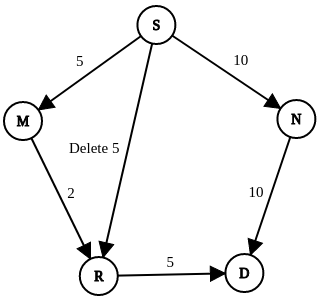
\includegraphics[scale=0.4]{img/Delete2.png}    
\end{center}
In the above graph the Optimal Path before deletion was $S \rightarrow R \rightarrow D$, when we delete the edge $S \rightarrow R$, the Optimal Path changes to $S \rightarrow M \rightarrow R \rightarrow D$.\\
Below we prove some important properties that holds when we remove edges from graph. The following properties holds when we have the Optimal Path for the graph before deletions.\\
\\
\hypertarget{Lemma 6}{\textbf{Lemma 6:}} \textit{Deletion of edge $ u \rightarrow v$ where $u \in V$ and $v \in V$ can not decrease $f(v)$.}\\
\textbf{Proof:} Let edge $ u \rightarrow v$ gets deleted from graph then,
\begin{itemize}[label={}]
    \item \textit{Case 1:} If $u =$ optimal\_parent($v$) then, source $\rightarrow u \rightarrow v$ was the optimal path of reaching $v$ from source, So after deletion, $f(v)_{new} = g(s) + w_{sv} + h(v)$ where $s$ is parent of $v$ with least $g$, In A* we chose the path with least $f$ as we chose $u$ before $s$ implies $f(v)_{new} \geq f(v)_{old}$.\\
    
    \item \textit{Case 2:} If $u$ is  not the optimal\_parent($v$), then let $s$ be the optimal\_parent($v$), deletion of edge $u \rightarrow v$ doesn't affect the $f(v)$ as the least cost of reaching $v$ is from $s$.\\
\end{itemize}
From above we can say that deletion of edge $u \rightarrow v$ can only increase $f(v)$. Hence Proved.\\
\\
\hypertarget{Lemma 7}{\textbf{Lemma 7:}} \textit{If edge($u,v$) $\notin$ Optimal Path, then deletion of such edges doesn't affect the Optimal Path.}\\
\textbf{Proof:} Suppose we delete edge($u,v$) $\notin$ Optimal Path then, as from \hyperlink{Lemma 6}{\textit{Lemma 6}} deletion of such edges can only increase $f(v)$ so if there is a path from source $\rightarrow v \rightarrow$ destination then it's cost will be increased, as Optimal Path is least cost path such paths cannot be an Optimal Path, Hence deletion of such edges doesn't affect the Optimal Path.\\
\\
\hypertarget{Lemma 8}{\textbf{Lemma 8:}}\textit{If edge(u,v) is deleted and optimal\_parent(v)$\neq$u, then deletion of such edges doesn't affect the Optimal Path.}\\
\textbf{Proof:} If $u$ is  not the optimal\_parent($v$), then let $s =$ optimal\_parent($v$), deletion of edge $u \rightarrow v$ doesn't affect the $f(v)$ as the least cost of reaching $v$ is from $s$, as there is no change in cost of any nodes so Optimal Path remains same.

\subsection{Batch Deletion}
Instead of deleting edges one by one we process deletion in batches, where a batch contains all the deleted edges before an query. From \hyperlink{Lemma 6}{\textit{Lemma 6}} we know that deletion of edges can increase the optimal cost, to compute the new optimal cost, we first propagate the change in cost due to deletion of edges to all affected nodes and then we perform a check so that we  are not violating the \hyperlink{Lemma 1}{\textit{Lemma 1}} after propagation, which is a essential property to always hold so that later we can process the next incoming updates, if it violates \hyperlink{Lemma 1}{\textit{Lemma 1}} then we start A* from where we left before i.e using the open\_list we have computed before. At the end we will have the new Optimal Path with the optimal cost for new graph encompassing all the deletions.\\
\\
\textit{Propagation for Deletion:}
\begin{enumerate}
    \item For each deleted edge $u \rightarrow v$, if $f(v) \neq \infty$ and optimal\_parent($v$)$=u$ then for such edges we compute the cost of reaching $v$ from its parent's and chose the least one as optimal\_parent($v$) and update $f(v)$, if $v$ doesn't have any parent then $f(v)=\infty$, and we add $v$ to update\_list.
    
    \item For each child of nodes in update\_list, we compute the cost $f$ of child with respect to node and If new cost $f$ is more than $f(child)$ and optimal\_parent(child)  is node then,we compute the cost of reaching child from all of its parents and update $f$ to the least cost of the parents and set that parent as optimal\_parent. And we add child to next update\_list.
    
    \item We repeat step 1 and 2 until update\_list is empty.
\end{enumerate}
Optimal Cost is least cost of reaching the node but we increase the cost of child at step 2 in above procedure, why we do that is because from \hyperlink{Lemma 6}{\textit{Lemma 6}} we know that $f$ might increase due to deletion of edges and we need to propagate the updated higher cost. Also since there is no special ordering of nodes to execute the propagation it may happen that while we propagating for a node its sub-graph might already have been updated so to make sure we have latest cost value among those, we choose the least cost parent and then propagate that cost downwards if applicable.\\ 
\begin{center}
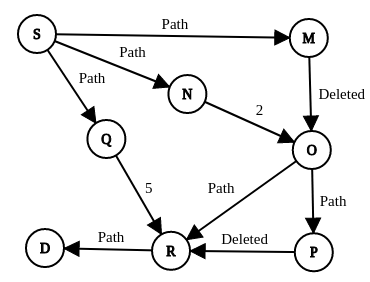
\includegraphics[scale=0.45]{img/Delete1.png}    
\end{center}
In above example the Optimal Path before deletion is $S \rightarrow M \rightarrow O \rightarrow P \rightarrow R \rightarrow D $.
The edges $ M \rightarrow O$ and $P \rightarrow R$ are deleted from graph. So $R,O \in $ update\_list, While propagating for $O$ we might find $R$ again from path $O \rightarrow R$ but $R$ has already updated, if in that update $R$ has chosen path $S \rightarrow M \rightarrow O \rightarrow R$ as its Optimal Path then we have stale value for $f(R)$ as $M \rightarrow O$ is deleted but since $R$'s update happened first it read the stale value before propagation. In such cases we need to find the parent with least cost thus we compute the cost of reaching node from all its parent and choose the parent with least cost as optimal\_parent.

\subsection{Deletion and Cycles}
We propagate the deletions so that each node whose cost is already computed will have the latest value. There is a special case of deletions with cycle where even after propagation we can get stale value if we don't perform  certain checks while propagating latest value to nodes. as given in example below:
\begin{center}
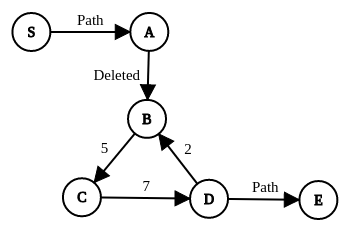
\includegraphics[scale=0.45]{img/cycle.png}        
\end{center}
In The above example the Optimal Path is from $S \rightarrow ABCD \rightarrow E$,where $S$ is source and $E$ is destination. When we remove the edge $A \rightarrow B$, and recompute the $f(B)$, there exist only one parent $D$ so the $f(B)_{new}$ is computed by $f(B)_{new} = g(D) + 2 + h(B)$, which is old value of $g(D)$, as we remove $A \rightarrow B$, there is no path from $S \rightarrow D$ so $g(D)_{new}$ is $\infty$, but we never arrive at that proposition because in propagation of deletion we will propagate from $B$  and $f(D)$ will be updated based on stale value of $f(B)$ and thus we have wrong cost value after deletion of such edges. The main reason this happens is die to the fact that cost $f(D)$ is computed wrt $B$ as $B \in OptimalPath(S,D)$. To avoid such cases, while chosing the optimal\_parent we have to eliminate the parents whose Optimal\_ancestor is current node.\\
\begin{lstlisting}[language=python, caption=Check Cycles]
procedure: check_cycle(node,parent):
    current_node = node
    while there exists optimal_parent(current_node):
        if current_node == parent:
            return true
        current_node = optimal_parent(current_node)
    
    return false
\end{lstlisting}

\subsection{Parallel Deletion and Cycle}
When there are multiple deletions happening at same time, there can be cycle of optimal\_parent, and thus when we do the above check, we get into an infinite loop also we defined optimal\_parent as a non cyclic path to start node. To eliminate such cycle when we process deletion we have to do additional processing of removing such cycles.\\
\begin{center}
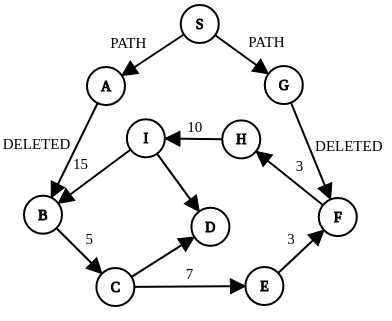
\includegraphics[scale=0.45]{img/Delete_cycle.png}        
\end{center}
In the example graph given above, the Optimal Path from $S\rightarrow D$ is $SABCD$,when we delete edges $A \rightarrow B$ and $G \rightarrow F$,for node $B$ the new parent is $I$ as $B \notin optimal\_parents(I)$, also the new parent of $F$ becomes $E$ as $E \notin optimal\_parents(F)$ this is because we are checking for optimal\_parent for both nodes in parallel thus the check happens at the same time and both reads the optimal\_parent values before it gets changed by either one of them. Thus forming a cycle of optimal\_parents which violates our definition of optima\_parent, to solve this we perform additional cycle check after each iteration of propagation for deletion and if such cycle found we remove them.\\
Now the question arises to remove which newly formed edge of the cycle i.e remove $I= $optimal\_parent($B$) or remove $E=$ optimal\_parent($F$). which one belongs to the optimal path? the answer is we can just remove any of cycle edges and our propagation algorithm will take care of which edge actually belong to the cycle.\\

%explain HOW

The propagation for deletion handling all the above cases is given below:
\begin{lstlisting}[language=python, caption=Propagation of Deletions]
procedure: propagate_deletions( list< pair<u,v> > Deletions, E, N):
     update_list = make_update_list(Deletions);
     check_optimal_parent_cycle(update_list);
     
     while update_list not empty:
        s = size(update_list)
        #array of N elements initialized to 0
        flag = array(N,0)
        #s parallel
        expand(update_list,s,flag)
        
        #create update list from flag
        update_list = generate_update_list(flag)
        
        #remove optimal_parent cycle 
        check_optimal_parent_cycle(update_list);

#GPU kernel
procedure: expand(update_list,s,flag):
    id = global_thread_id;
    node = update_list[id];
    
    for each child ch of node:
        lock(ch)
        
        if f(ch) > g(node) + weight(node,ch) + h(ch):
            f(ch) = g(node) + weight(node,ch) + h(ch)  
            optimal_parent[ch] = node
            flag[ch] = 1
        
        else if f(ch) < g(node) + weight(node,ch) + h(ch) and optimal_parent[ch] == node:
            for all parents p of ch:
            
                if check_cycle(ch,p) == true:
                    continue
            
                if f(ch) > g(p) + weight(p,ch) + h(ch):
                    f(ch) = g(p) + weight(p,ch) + h(ch)
                    optimal_parent[ch] = p
            
            flag[ch] = 1
        
        unlock(ch)
        
\end{lstlisting}
\hypertarget{Lemma 9}{\textbf{Lemma 9:}} \textit{At the end of propagation for deletion all node  $ n \in V$  such that $f(n)_{old} \neq \infty $ has the latest $f(n)$ which is optimal cost in new graph including deletions. }\\
\textbf{Proof:} Suppose we delete edge $u \rightarrow v$. Let node $n \in V$:\\
\textit{Case 1:} If $n \in$ sub-graph($v$) then there can be two sub-cases: \begin{enumerate}
\item If $v \in$ Optimal\_Path($n$) which implies $f(n) \neq \infty$, when we add $v$ in update\_list we compute the least cost of reaching $v$ from all of its remaining parent we also make sure that the parent we chose is such that its cost in not computed wrt $v$ which implies its the optimal\_cost of reaching $v$. Since $v \in$ Optimal\_Path($n$) , $\exists$ parent $p$ of $n$ such that $p \in$ Optimal\_Path($n$) and $p \in$ sub-graph($v$), which implies $p \in$ update\_list at some iteration of propagation, when $p$ tries to update $n$, $n$ will chose the best available parent thus cost of $f(n)$ is optimal\_cost of reaching $n$ in new graph.
\item If $v \notin$ Optimal\_Path($n$),then $\exists$ optimal\_parent $p$ such that $v \notin $ Optimal\_Path($p$), thus $n \notin$ update\_list at any iteration of propagation so $f(n)$ remains same which is the optimal\_cost from \hyperlink{Lemma 7}{\textit{Lemma 7}}. 
\end{enumerate}
\textit{Case 2:} If $n \notin$ sub-graph($v$) then $v \notin$ Optimal\_Path($n$) also $v \notin$ update\_list at any iteration of propagation so $f(n)$ remains same which is the optimal\_cost from \hyperlink{Lemma 7}{\textit{Lemma 7}}\\
\\
\textbf{Claim:} \textit{At the end of propagation $f(destination)$ might not be the optimal cost of reaching destination from source in new graph. }\\
\textbf{Proof:}
\begin{center}
    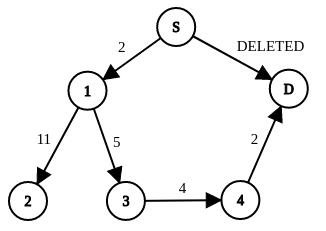
\includegraphics[scale=0.4]{img/del_prop.png}
\end{center}
To prove, It is sufficient to give an example where $f(destination)$ is not the optimal cost after propagation for deletion.\\
In above graph at end of A* we will have:\\
open\_list : \{2,3\}\\
closed\_list : \{S,1,D\}\\
Thus node 4 is not visited thus having $f(4)=\infty$, after propagation for deletion as D has only one parent 4 its cost is computed wrt 4 so $f(D)=\infty$, but int the new graph the optimal cost is $f(D)=13$ with Optimal\_Path $S\rightarrow 1\rightarrow 3 \rightarrow 4 \rightarrow D$.\\
Thus in above graph $f(D)$ after the propagation of deletion is not the optimal cost in new graph.\\
\\
\hypertarget{Lemma 10}{\textbf{Lemma 10:} }\textit{After propagation of deletions if $f(destination) < f(n)$ $ \forall$ $n \in $open\_list then $f(destination)$ is the optimal cost of reaching destination from source.}\\
\textbf{Proof:} $\forall$ node $n \in $ open\_list $f(n)_{old} \neq \infty$ so from \hyperlink{Lemma 9}{\textit{Lemma 9}} after propagation of deletion $n$ has the optimal\_cost $f(n)$ in new graph. Also given $f(destination) < f(n)$ $ \forall$ $n \in $open\_list, As weights are non-negative so for all descendants of $n$ $f($ descendants $) > f(n)$. So reaching $destination$ from any node in update\_list will have larger cost than current value, thus $f(destination)$ is the optimal cost reaching destination from source.\\
\\
From \textit{Claim} made above we know that after propagation for deletion $f(destination)$ is not the optimal cost, also from \hyperlink{Lemma 10}{\textit{Lemma 10}} we know that if $f(destination) < f(n)$ $ \forall$ $n \in $ open\_list then $f(destination)$ is the optimal cost, to satisfy the this condition we need to perform A* after propagation for deletion as after A* $f(destination) < f(n)$ $ \forall$ $n \in $open\_list and thus $f(destination)$ is the optimal cost.
\begin{lstlisting}[language=python, caption=Manage Deletions]
procedure: Deletions(list< pair<u,v> > deleted_edges,N,E)
    propagate_deletions(deleted_edges,N,E);
    # A* from old saved state
    GA*(open_list,closed_list,source,destination,K)

\end{lstlisting}
%explanation about why we need A* after this.
\section{Fully Dynamic}
Real world graphs are dynamic and edges are changing continuously so there are insertion of edges and deletion of edges at same instance in such cases if a query is raised to find the optima path from source to destination we can retrieve the optimal path without re-executing A* from start again.

\subsection{Separate Propagation }
As we have already discussed how to find the optimal path when edges are either added only or deleted only we can infer the dynamic change in edges at a single instance as addition happening first then deletion or vice versa. So we process addition first as insertion only then we process deletion as deletion only. It may happen that some nodes will get updated multiple times in two different propagation. But as insertion and deletion require different set of instruction it is a good choice to separate the propagation.
\begin{lstlisting}[language=python, caption=Separate Propagation]
procedure: separate_propagation(list< pair<u,v> > inserted_edges,list< pair<u,v> > deleted_edges,N,E)
    propagate_insertions(inserted_edges,N,E)
    propagate_deletions(deleted_edges,N,E)
    # A* from old saved state
    GA*(open_list,closed_list,source,destination,K)
\end{lstlisting}
\hypertarget{Lemma 11}{\textbf{Lemma 11:}} \textit{After separate propagation $f(destination)$ is the optimal cost of reaching destination from source in new graph including insertion and deletions.}\\
\textbf{Proof:} In separate propagation first we propagate for insertions and as from \hyperlink{Lemma 5}{\textit{Lemma 5}} at end of it we have $f(destination)$ as the optimal cost in new graph which just includes all inserted edges.
In the new graph we propagate for deletions and then perform GA* so from \hyperlink{Lemma 10}{\textit{Lemma 10}} we have $f(destination)$ as the optimal cost in the graph which include both insertion and deletion. Thus $f(destination)$ is the optimal cost of reaching destination from source in new graph including insertion and deletions.

\subsection{Simultaneous Propagation}
We have designed the propagation of Insertion( section 4) and propagation of deletions (section 5) such some part of them can be overlapped and we can process both insertion and deletion at same time by considering them as an update. But since both propagation are happening at same time there are few additional cases we need to take care of thus adding some more checks as given below.

\subsubsection{Insert-Delete Cycle}
Since we have insertions and deletions propagating at same time, If we don't perform enough checks we can get into cycles for certain cases. 
\begin{center}
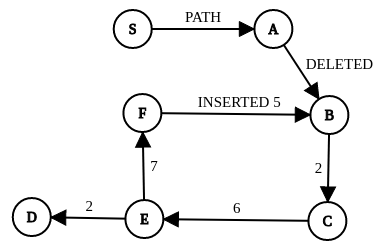
\includegraphics[scale=0.45]{img/ins_del_cycle.png}        
\end{center}
In the example graph given above we remove $A \rightarrow B$ and insert $F \rightarrow B$, Due to deletion $f(B) = \infty$, when we propagate for edge $F \rightarrow B$,the cost of reaching $B$ from $F$ via newly added edge is less than infinity thus, we compute the new cost and make optimal\_parent($B$) = $F$,But when we try to to retrace the path from $F$ to $S$ we get $F\rightarrow E\rightarrow C\rightarrow B\rightarrow F...$ thus we have a optimal\_parent cycle. It is because the cost of $F$ itself is a stale value due to the fact that its cost is computed wrt to $B$ and deleted edge $A \rightarrow B$. To remove such cases we have to extensively check for insertion of edges $u \rightarrow v$, if $v \in $optimal\_parents($u$) for all insertions.\\

\subsubsection{Propagation Cycle}
Since Insertions and Deletions are propagating at same if there is cycle and each the reach the cycle at diff iterations, It might happen due to structure of graph that they propagate indefinitely on such cycles if the check mentioned in the above section is not implemented for each insertion.  

\begin{center}
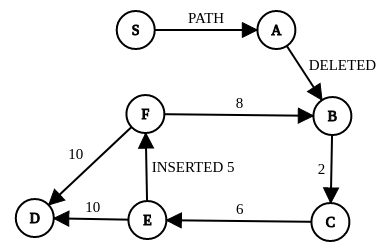
\includegraphics[scale=0.45]{img/prop_cycle.png}        
\end{center}

In the example above $A \rightarrow B$ is deleted and $E \rightarrow F$ is added. Due to deletion cost of $B = \infty$  and due to insertion cost of $F$ is changed in next iteration cost of $C = \infty$ as there is no path from $S \rightarrow C$ in new graph, also due to edge $f \rightarrow B$ the cost of $B$ is changed as the new cost is less than $\infty$. In the next iteration cost of $E = \infty$ and cost of $C$ is changed ,Similarly in next iteration cost of $F = \infty$ and cost of $E$ is changed, and similarly the propagation goes on the loop indefinitely. The problem here is we computed cost of $B$ from $F$ when $F$ has the stale value and its cost is computed wrt $B$ itself. This can be removed by doing check mentioned in above section 4.2.1. 

\begin{lstlisting}[language=python, caption=Propagation of Updates]
procedure: propagate_updates( list< pair<u,v> > Deletions,list< pair<u,v> > Inserts, E, N):
     update_list = make_update_list_insertion(Inserts);
     update_list = append( update_list, make_update_list_deletion(Deletions) )
     
     while update_list not empty:
        s = size(update_list)
        #array of N elements initialized to 0
        flag = array(N,0)
        #s parallel
        expand(update_list,s,flag)
        #create update list from flag
        update_list = generate_update_list(flag)

#GPU kernel
procedure: expand(update_list,s,flag):
    id = global_thread_id;
    node = update_list[id];
    
    for each child ch of node:
        lock(ch)
        
        if f(ch) > g(node) + weight(node,ch) + h(ch):
            f(ch) = g(node) + weight(node,ch) + h(ch)  
            optimal_parent[ch] = node
            flag[ch] = 1
        
        elif f(ch) < g(node) + weight(node,ch) + h(ch) and optimal_parent[ch] == node:
            for all parents p of ch:
             
                if check_cycle(ch,p) == true:
                    continue
             
                if f(ch) > g(p) + weight(p,ch) + h(ch):
                    f(ch) = g(p) + weight(p,ch) + h(ch)
                    optimal_parent[ch] = p
            
            flag[ch] = 1
        
        unlock(ch)
\end{lstlisting}

% \textbf{Lemma 12:} \textit{After  simultaneous propagation of updates if $f(destination) < f(n)$ $ \forall$ $n \in $open\_list then $f(destination)$ is the Optimal Cost of reaching destination from source.}

\section{Experimental Results}
%results

The performance of GA* \cite{GA*} is dictated by how much parallelism we can create i.e number of parallel threads that we can spawn which is equal to the number of priority queues (K). As the we increase the number of priority queues the execution time decreases because we get benefited from GPU's SIMD architecture. The trend follows as shown in graph below.
\begin{center}
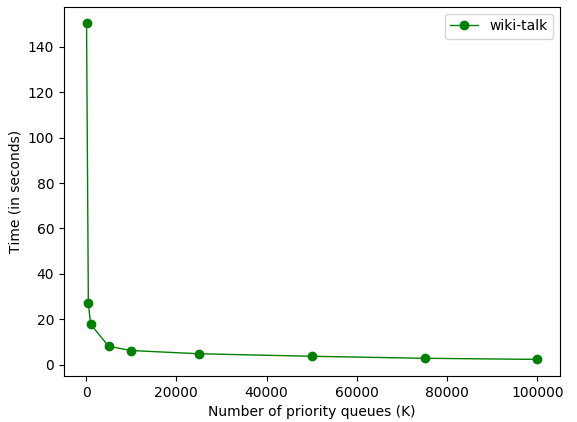
\includegraphics[scale=0.45]{img/RvK.png}        
\end{center}
For Insertion only the amount of processing required is directly proportional to the number edges inserted in graph. As we increase the number of edges inserted the execution time increase, Its not a steady increase because the probability that a node is getting updated due to multiple propagation increases thus the contention at lock of that node increases slowing the execution time.
\begin{center}
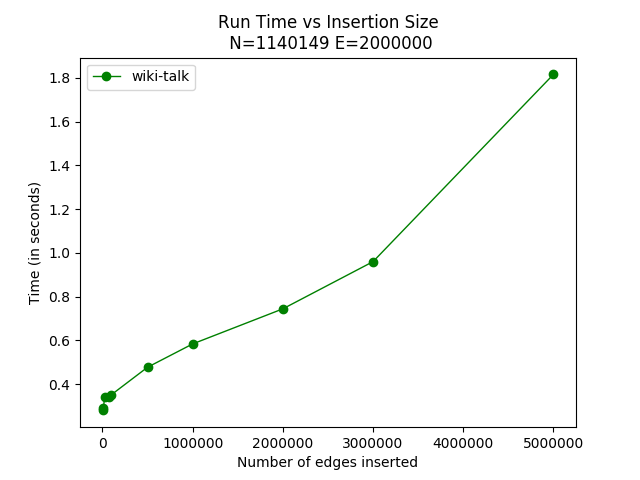
\includegraphics[scale=0.45]{img/IvK.png}        
\end{center}
Similarly for deletion as deletion size increases we need to process more nodes,and contention at lock also increases thus increasing the execution time, as shown in graph below.
\begin{center}
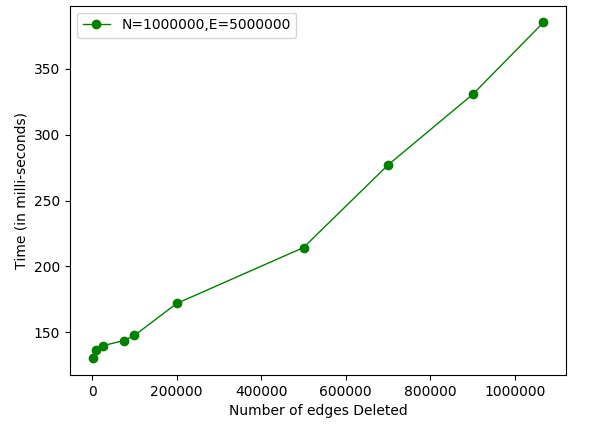
\includegraphics[scale=0.45]{img/DvT.png}        
\end{center}
In dynamic setting when we process both insertion and deletion at same time, the amount of execution time needed to process deletion is much larger than inserts. As shown in below graph where the total number of updates are kept constant but the amount of updates which are insertion or deletion is changed we see that there is a drastic drop in execution time as the percentage of deletion becomes 0. It shows that even for small amount of deletion the execution time is high compared to insertions. It is because we are performing multiple checks for cycle when we process deletion which takes a major amount of execution time, while in insertion there is no need to check for cycle when we are doing separate propagation.\\
\begin{center}
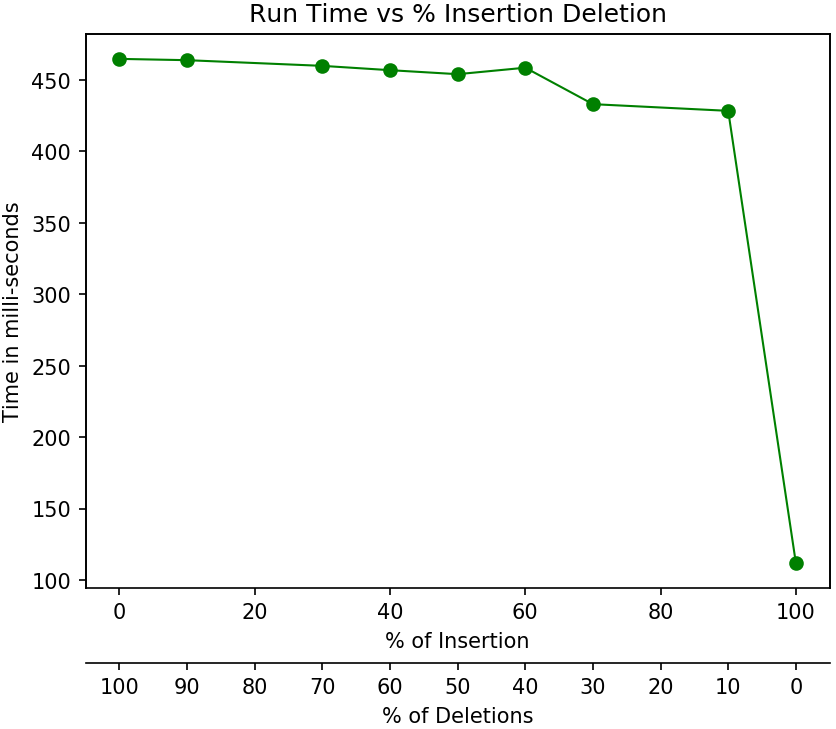
\includegraphics[scale=0.45]{img/IDvK.png}        
\end{center}
The method we proposed for handling insertion and deletion rather than re-doing A* from beginning is much faster then later. The below two graph shows how execution time varies when we increase the number of queries ( finding path from source to destination after some update ) increases. Performing  GA* after each set of updates is almost linear but propagating the updates as described in above sections takes considerably less amount of execution time. The speed up we can get is proportional to the number of queries we preform, as the number of queries increases we get better and better speed up. In the graph shown below the graph on left side updates only consist of \textit{inserts} while the graph on right has update consisting of both insertion and deletion. In the graph on right we can infer that when number of queries is 1 multiple GA* perform better than Dynamic A* but as we increase the number of queries Dynamic A* perform better than multiple GA*.
\begin{center}
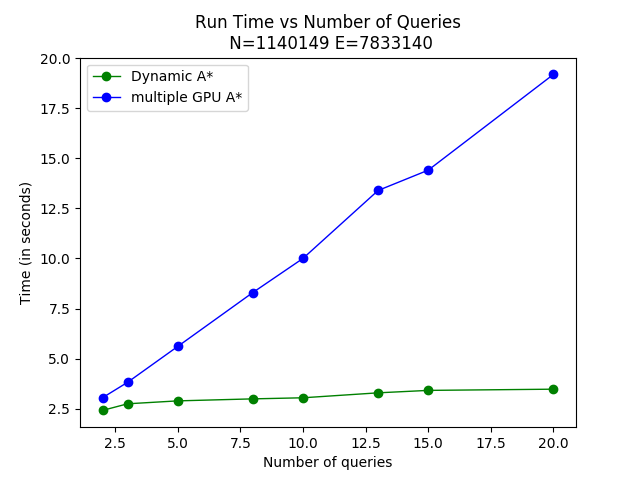
\includegraphics[scale=0.36]{img/TvQ_wikitalk.png}        
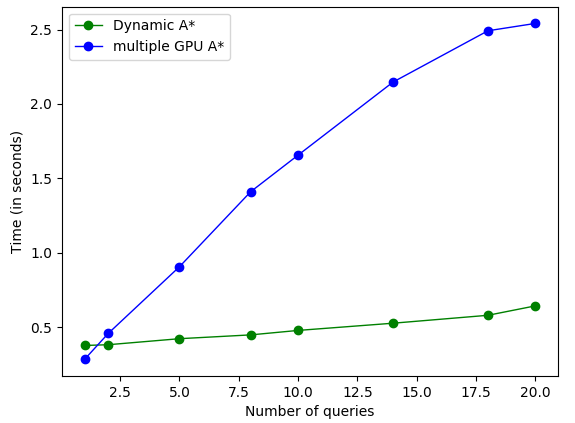
\includegraphics[scale=0.36]{img/QvT_dyn.png} 
\end{center}



\section{Related Work}
A* \cite{A*} is one of the widely used path-finding algorithm, Peter Hart, Nils Nilsson and Bertram Raphael of Stanford Research Institute (now SRI International) first published the algorithm in 1968. It can be seen as an extension of Dijkstra's algorithm where $h(x)=0 $ $\forall x, x \in V$. A* achieves better performance by using heuristics to guide its search. What makes it different from greedy best-first algorithm is it takes already travelled distance $g(x)$ into account.\\
D*\cite{original D*}, focused D*\cite{focused D*} and D* lite\cite{D* Lite} are a family of incremental search algorithms. The original D*\cite{original D*} by Anthony Stentz, is an informed incremental search algorithm. Focussed D*\cite{focused D*} is an informed incremental heuristic search algorithm by Anthony Stentz that combines ideas of A*\cite{A*} and the original D*\cite{original D*}. Focussed D* resulted from a further development of the original D*. D* Lite \cite{D* Lite} is an incremental heuristic search algorithm by Sven Koenig and Maxim Likhachev that builds on LPA*\cite{LPA*}, an incremental heuristic search algorithm that combines ideas of A* and Dynamic SWSF-FP \cite{SPP}. All three search algorithms solve the same assumption-based path planning problems, including planning with the free space assumption\cite{PF} where a robot has to navigate to given goal coordinates in unknown terrain. So in all the three algorithms the graph is changing while we try to find the shortest path to the destination, this is a major difference between our Dynamic A* in D* as we try to find the shortest path to destination after some changes(insertion + deletion) has occurred since our last search. Other major change is in D* only the cost of edges are changed while the number of edges remains fixed But in our case edges can be removed as well as added and the cost change can be emulated as deleting that edge and later adding the same edge with new cost. The name D* comes from the term "Dynamic A*", because the algorithm behaves like A* except that the arc costs can change as the algorithm runs.\\

\section{Conclusion and Future Work}
We have proposed algorithm which can efficiently find optimal path with the help of heuristics on GPU while taking account for updates in form of insertion and deletions with time. Our algorithm is faster than doing repeated A* on GPU from scratch. We also found that insertions takes less time to process than deletion. And due to the fact that both insertion and deletion requires different set of instruction to process, separate propagation outperforms simultaneous propagation.\\
In future the possibility of Dynamic A* in multi-GPU environment can also be explored. There can be algorithmic development in dynamic bi-directional A* on GPU. \newpage
\begin{thebibliography}{} 
    \bibitem{A*} Hart, P.; Nilsson, N.; Raphael, B. (1968), "A Formal Basis for the Heuristic Determination of Minimum Cost Paths", IEEE Trans. Syst. Science and Cybernetics
    \bibitem{original D*}Stentz, Anthony (1994), "Optimal and Efficient Path Planning for Partially-Known Environments", Proceedings of the International Conference on Robotics and Automation
    \bibitem{focused D*}Stentz, Anthony (1995), "The Focussed D* Algorithm for Real-Time Replanning", Proceedings of the International Joint Conference on Artificial Intelligence
    \bibitem{D* Lite}Koenig, S.; Likhachev, M. (2005), "Fast Replanning for Navigation in Unknown Terrain", Transactions on Robotics
    \bibitem{LPA*}Koenig, S.; Likhachev, M.; Furcy, D. (2004), "Lifelong Planning A*", Artificial Intelligence.
    \bibitem{GA*}Yichao Zhou and Jianyang Zeng (2015): Massively Parallel A* Search on a GPU, Twenty-Ninth AAAI Conference on Artificial Intelligence.
    \bibitem{Diff CSR}Gaurav Malhotra, Hitish Chappidi, Rupesh Nasre(2016): Fast Dynamic Graph Algorithms.
    \bibitem{SPP} Ramalingam, G.; Reps, T. (1996), "An incremental algorithm for a generalization of the shortest-path problem", Journal of Algorithms
    \bibitem{PF}Koenig, S.; Smirnov, Y.; Tovey, C. (2003), "Performance Bounds for Planning in Unknown Terrain", Artificial Intelligence
    \bibitem{Giuseppe}Giuseppe F. Italiano: Dynamic Graph Algorithms.
    \bibitem{Wiki A*}\texttt{https://en.wikipedia.org/wiki/A*\_search\_algorithm}
    \bibitem{Wiki D*}\texttt{https://en.wikipedia.org/wiki/D*}
    
\end{thebibliography}


% All reduce Graphs
\newpage 
    \section{Appendix} 
    \subsection{Heuristics in A*}
     Performance of A* depends heavily on the type of heuristics which is used. It guides the search to reach destination faster,but wrong values can also lead to slower or a path which is not the shortest path.
     $\forall x \in V$
     \begin{itemize}
         \item If $h(x)=0$, then A* turns into in Dijkstra's Algorithm.
         \item If $h(x) \leq$ cost of reaching destination from x, We are guaranteed to find the shortest path but it will be slower.
         \item If $h(x) = $cost of reaching destination from x, we will follow only the best path.
         \item If $h(x)$ is sometimes greater than cost of reaching destination from $x$. A* is not guaranteed to find the shortest path.
         \item If $h(x)>> g(x)$, then only $h(x)$ plays a role and A* turns into greedy best first search.
     \end{itemize}
    Considering the above factors in our implementation for general graphs we chose $h(x)$ as bfs distance from destination to $x$, so we are always guaranteed to find the shortest path.
    % \subsection{Storing dynamic Graph on GPU}
    % \subsection{Global Lock in GPU}
    

% Lockin implementation, K PQ implemetation, GA* implementation

\end{document}